
%%%%%%%%%%%%%%%%%%%%%%%%%%%%%%%%%%%%%%%%%%%%%%%%%%%%%%%%%%%%%%%%%%%%%%%
%%%%%%%%%%%%%%%%%%%%%%%%%%%%%%%%%%%%%%%%%%%%%%%%%%%%%%%%%%%%%%%%%%%%%%% 
%%%%%%%%%%%       								 Preamble				         	                                                        %%%%%%%%%% 
%%%%%%%%%%%%%%%%%%%%%%%%%%%%%%%%%%%%%%%%%%%%%%%%%%%%%%%%%%%%%%%%%%%%%%% 
%%%%%%%%%%%%%%%%%%%%%%%%%%%%%%%%%%%%%%%%%%%%%%%%%%%%%%%%%%%%%%%%%%%%%%% 
\documentclass[10pt]{beamer}
\usepackage{setspace}
\usepackage{color}
\usepackage{amsmath,lmodern}
\usepackage{hyperref}
\usepackage{graphicx}
\usepackage{multirow}
\usepackage{tikz}
\usetikzlibrary{fit,shapes.misc}
\usepackage{pdflscape}
\usepackage{amsmath}
\usepackage{lscape}
\usepackage{multirow}
\usepackage{enumerate}
\usepackage{epstopdf}
\usepackage{pdfpages}
\usepackage{appendixnumberbeamer}
\usepackage{color,soul}
\usepackage{grffile}
\usepackage{float}
\usepackage{relsize}
\usepackage{tcolorbox}
\newcounter{nodemarkers}
\usepackage{tikz}
\newcommand{\toplinesmall}{%
  \tikz[remember picture,overlay] {%
    \draw[blue,thick] ([yshift=-1cm, xshift=.9cm]current page.north west)
             -- ([yshift=-1cm,xshift=3.6cm]current page.north west);}}
             
\newcommand{\toplinemedium}{%
  \tikz[remember picture,overlay] {%
    \draw[blue,thick] ([yshift=-1cm, xshift=.9cm]current page.north west)
             -- ([yshift=-1cm,xshift=6.2cm]current page.north west);}}
 
 \newcommand{\toplinelarge}{%
  \tikz[remember picture,overlay] {%
    \draw[blue,thick] ([yshift=-1cm, xshift=.9cm]current page.north west)
             -- ([yshift=-1cm,xshift=8.9cm]current page.north west);}}           
             
 \newcommand{\toplinexlarge}{%
  \tikz[remember picture,overlay] {%
    \draw[blue,thick] ([yshift=-1cm, xshift=.9cm]current page.north west)
             -- ([yshift=-1cm,xshift=12cm]current page.north west);}}                       
             
\setbeamertemplate{footline}
{
  \leavevmode%
  \hbox{%
  \begin{beamercolorbox}[wd=.333333\paperwidth,ht=2.25ex,dp=1ex,center]{author in head/foot}%
    \usebeamerfont{author in head/foot}{\textcolor{blue}{ECON311}}
  \end{beamercolorbox}%
  \begin{beamercolorbox}[wd=.333333\paperwidth,ht=2.25ex,dp=1ex,center]{title in head/foot}%
    \usebeamerfont{title in head/foot}{\textcolor{blue}{Winter 2026}}
  \end{beamercolorbox}%
  \begin{beamercolorbox}[wd=.333333\paperwidth,ht=2.25ex,dp=1ex,right]{date in head/foot}%
    \usebeamerfont{date in head/foot}{\textcolor{blue}{Lecture 5 \: \: \: \: \: \: \: }
    \insertframenumber{} / \inserttotalframenumber\hspace*{2ex}} 
  \end{beamercolorbox}}%
  \vskip0pt%
}
\newtheorem{proposition}[theorem]{Proposition}

\newcommand\marktopleft[1]{%
    \tikz[overlay,remember picture] 
        \node (marker-#1-a) at (-0.2,1.2ex) {};%
}
\newcommand\markbottomright[1]{%
    \tikz[overlay,remember picture] 
        \node (marker-#1-b) at (0.16,-1ex) {};%
    \tikz[overlay,remember picture,thick,inner sep=4pt]
        \node[draw,rectangle,rounded corners, blue, fit=(marker-#1-a.center) (marker-#1-b.center)] {};%
}

\setbeamertemplate{caption}{\raggedright\insertcaption\par}
\setbeamertemplate{itemize items}[ball]
\setbeamertemplate{itemize subitem}[triangle]
\setbeamertemplate{itemize subsubitem}[triangle]
\tcbset{colframe=white,colback=white,nobeforeafter}
\beamertemplatenavigationsymbolsempty
\addtobeamertemplate{frametitle}{\vspace*{0.19cm}}{\vspace*{0cm}}


%%%%%%%%%%%%%%%%%%%%%%%%%%%%%%%%%%%%%%%%%%%%%%%%%%%%%%%%%%%%%%%%%%%%%%%
%%%%%%%%%%%%%%%%%%%%%%%%%%%%%%%%%%%%%%%%%%%%%%%%%%%%%%%%%%%%%%%%%%%%%%% 
%%%%%%%%%  									    Define Title									                                       %%%%%%%%%
%%%%%%%%%%%%%%%%%%%%%%%%%%%%%%%%%%%%%%%%%%%%%%%%%%%%%%%%%%%%%%%%%%%%%%%
%%%%%%%%%%%%%%%%%%%%%%%%%%%%%%%%%%%%%%%%%%%%%%%%%%%%%%%%%%%%%%%%%%%%%%% 
\title{ECON 311} 
\author{Lecture 5: Modeling Economic Growth}
\date{}
\AtBeginSection[]
{
 \begin{frame}<beamer>
 \tableofcontents[currentsection]
 \end{frame}
}
%%%%%%%%%%%%%%%%%%%%%%%%%%%%%%%%%%%%%%%%%%%%%%%%%%%%%%%%%%%%%%%%%%%%%%%
%%%%%%%%%%%%%%%%%%%%%%%%%%%%%%%%%%%%%%%%%%%%%%%%%%%%%%%%%%%%%%%%%%%%%%% 
%%%%%%%% 						     				Document								                                                %%%%%%%%
%%%%%%%%%%%%%%%%%%%%%%%%%%%%%%%%%%%%%%%%%%%%%%%%%%%%%%%%%%%%%%%%%%%%%%%
%%%%%%%%%%%%%%%%%%%%%%%%%%%%%%%%%%%%%%%%%%%%%%%%%%%%%%%%%%%%%%%%%%%%%%% 
\begin{document}
\setbeamercovered{transparent}

\begin{frame}
\maketitle
\end{frame}

%%%%%%%%%%%%%%%%%%%%%%%%%%%%%%%%%%%%%%%%%%%%%%%%%%%%%%%%%%%%%%%%%%%%%%%
%%%%%%%%%%%%%%%%%%%%%%%%%%%%%%%%%%%%%%%%%%%%%%%%%%%%%%%%%%%%%%%%%%%%%%% 
%%%%%%%% 						     				Introduction	             		                                		  %%%%%%%%
%%%%%%%%%%%%%%%%%%%%%%%%%%%%%%%%%%%%%%%%%%%%%%%%%%%%%%%%%%%%%%%%%%%%%%%
%%%%%%%%%%%%%%%%%%%%%%%%%%%%%%%%%%%%%%%%%%%%%%%%%%%%%%%%%%%%%%%%%%%%%%% 


\section{A Production Model}

\begin{frame}
\frametitle{\: \: \: Introduction}
\toplinemedium
\begin{itemize}
\item To understand the causes of the great differences in production across time and countries, we first write down the following  production function:
\begin{eqnarray*}
Y=F(K,L)=\overline{A}K^{\alpha}L^{(1-\alpha)} &, & \alpha \leq 1
\end{eqnarray*}  
\item This production function has several theoretical properties that facilitates the analysis of empirical implications of differences in $K$ and $L$.
\end{itemize}
\end{frame}

\begin{frame}
\frametitle{\: \: \: Properties of the Production Function}
\toplinexlarge
The Cobb-Douglas Production Function has the following properties:
\vspace{.15in}
\only<1>{
\begin{enumerate}
\item Diminishing returns to $K$ and $L$:
\end{enumerate}
\begin{columns}
\begin{column}{0.5\linewidth}
\begin{eqnarray*}
\begin{array}{l}
MPK=\frac{\partial Y}{\partial K}=\alpha \overline{A} \left( \frac{L}{K} \right)^{(1-\alpha)} \\[1.4ex]
MPL=\frac{\partial Y}{\partial L }=(1-\alpha) \overline{A} \left( \frac{K}{L} \right)^{\alpha}
\end{array}
\end{eqnarray*}
\end{column}
\begin{column}{0.5\linewidth}
\begin{figure}
\centering
\caption{Diminishing Returns to $i$ for $i=K,L$}
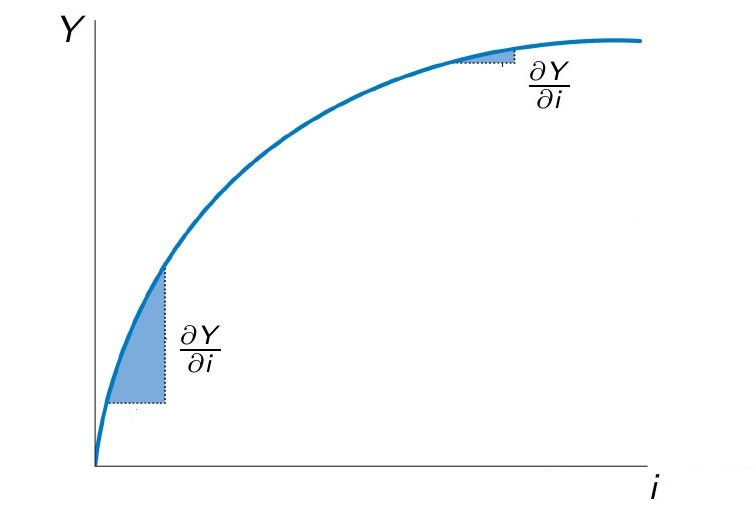
\includegraphics[scale=.28]{diminishing_returns}
\end{figure}
\end{column}
\end{columns}
\begin{itemize}
\item Differences in $K$ accumulation per person has different implications at different levels of development
\end{itemize}}
\only<2>{
\begin{enumerate}
\setcounter{enumi}{1}
\item Constant Returns to Scale:
\end{enumerate}
\begin{columns}
\begin{column}{0.5\linewidth}
\begin{eqnarray*}
\begin{array}{l}
F(\lambda K, \lambda L)=\lambda F(K,L) \\[1.4ex]
F(\lambda K, \lambda L)=\lambda \underbrace{\overline{A}K^{\alpha}L^{(1-\alpha)}}_{F(K,L)}
\end{array}
\end{eqnarray*}
\end{column}
\begin{column}{0.5\linewidth}
\begin{figure}
\centering
\caption{Constant Returns to scale}
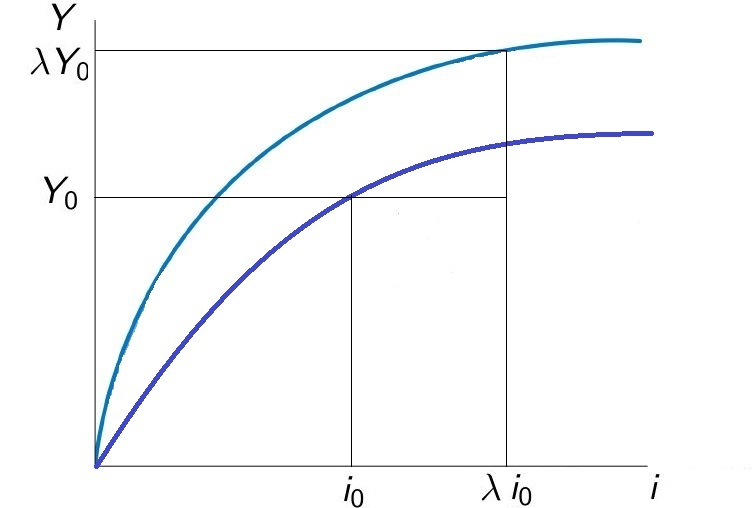
\includegraphics[scale=.28]{constant_returns_scale}
\end{figure}
\end{column}
\end{columns}
\begin{itemize}
\item Population size matters for total income but does not for income per capita
\end{itemize}}
\end{frame}

\begin{frame}
\frametitle{\: \: \: Solving for Production Parameters}
\toplinexlarge
\begin{itemize}
\item To take this model to the data, we need ...
\begin{itemize}
\vspace{.11in}
\item to assign value to the parameter, $\alpha$ 
\vspace{.11in}
\item and study how differences in the exogenous variables, $K$, $L$, $\overline{A}$, result in differences in endogenous variable, $Y$.
\end{itemize}
\vspace{.11in}
\item It turns out that from the optimal decision of firms to rent $K$ and hire $L$, we obtain:
\begin{eqnarray*}
\begin{array}{lcl} 
\frac{wL^*}{Y^*}=(1-\alpha) &, & \frac{rK^*}{Y^*}=\alpha
\end{array}
\end{eqnarray*}
\vspace{.11in}
\item We can obtain this from the income approach to measuring GDP: $\alpha=\frac{1}{3}$
\end{itemize}
\end{frame} 

\begin{frame}
\frametitle{\: \: \: Development Accounting}
\toplinelarge
\begin{itemize}
\item Our main concerned is to measure GDP per capita differences, so we expressed the production in per capita terms:
\begin{eqnarray*}
\begin{array}{lll}
y=\overline{A}k^{\frac{1}{3}} &, y=\frac{Y}{L}, &k=\frac{K}{L}
\end{array}
\end{eqnarray*}
\item We are going to assume that a country uses all of its resources to produce:
\begin{eqnarray*}
\begin{array}{lll}
k=\overline{k}&, &\overline{k}=\frac{\overline{K}}{\overline{L}}
\end{array}
\end{eqnarray*}
\item We observe differences in $\overline{k}$ but, because we do not observe differences in $\overline{A}$,...
\begin{itemize}  
\vspace{.11in}
\item we will assume that it is the same for all countries.
\end{itemize}
\vspace{.11in}
\item In the following exercise, we will calculate the output of country $c$ relative to the $US$:
\begin{eqnarray*}
\frac{y_c}{y_{US}}=\left(\frac{\overline{k}_{c}}{\overline{k}_{US}}\right)^{\frac{1}{3}}
\end{eqnarray*}
\end{itemize}  
\end{frame}

\begin{frame}
\frametitle{\: \: \: Development Accounting}
\toplinelarge
\begin{figure}
\centering
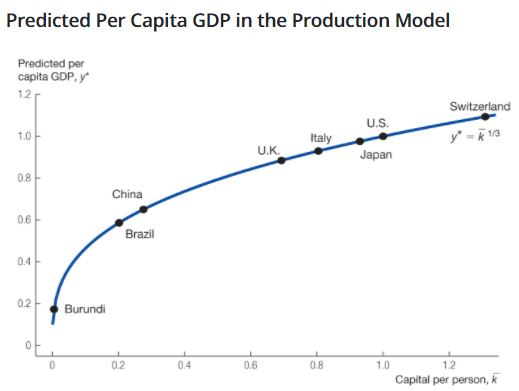
\includegraphics[scale=.65]{figure_44}
\end{figure}
\end{frame}

\begin{frame}
\frametitle{\: \: \: Development Accounting}
\toplinelarge
\begin{figure}
\centering
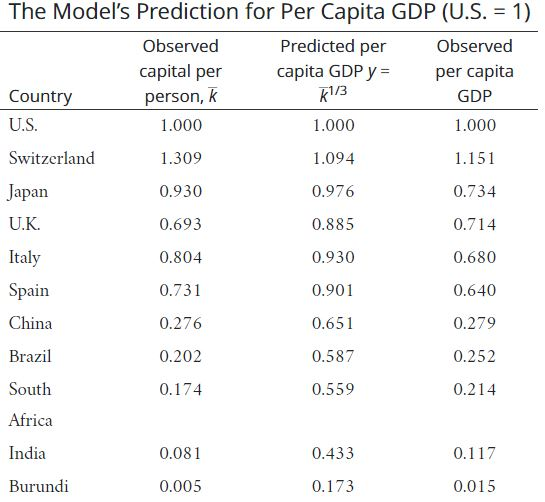
\includegraphics[scale=.48]{table_43}
\end{figure}
\end{frame}



\begin{frame}
\frametitle{\: \: \: Development Accounting}
\toplinelarge
\begin{figure}
\centering
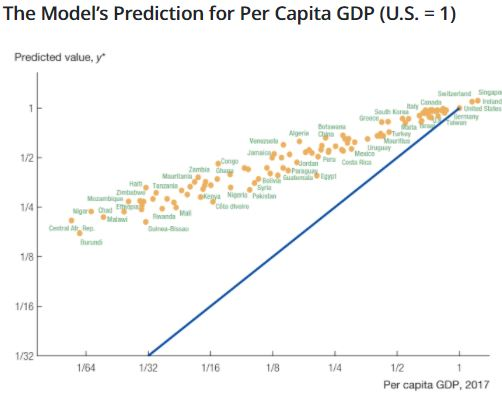
\includegraphics[scale=.65]{figure_45}
\end{figure}
\end{frame}

\begin{frame}
\frametitle{\: \: \:  Model with only $k$ and constant $\overline{A}$ }
\toplinexlarge
\begin{itemize}
\item The model without $\overline{A}$ differences underestimate differences in output per capita.
\vspace{.11in}
\item On average, $y$ in industrialized countries is 10 times larger than in non-industrialized countries:
\begin{eqnarray*}
10=\frac{\overline{A}^{ind}\left(k^{ind}\right)^{\frac{1}{3}}}{\overline{A}^{nind}\left(k^{nind}\right)^{\frac{1}{3}}} 
\end{eqnarray*}
\begin{itemize}
\item If we assume that $\overline{A}^{ind}=\overline{A}^{nind}$, then ...
\begin{eqnarray*}
10^3=1000=\frac{k^{ind}}{k^{nind}}
\end{eqnarray*}
\begin{itemize}
\item There is no empirical evidence of such large differences.
\end{itemize}
\end{itemize}
\vspace{.11in}
\item Presumably,  differences in $\overline{A}$ play a big role in accounting for differences in $y$.
\begin{itemize}
\vspace{.11in}
\item We cannot be certain of this because differences in $\overline{A}$ are unobserved in general.
\end{itemize}
\end{itemize}
\end{frame}





\begin{frame}
\frametitle{\: \: \: Understanding differences in $\overline{A}$}
\toplinelarge
\begin{itemize}
\item We could assume that our model is correct and interpret deviations of predicted  from observed as differences in $\overline{A}$.
\end{itemize}
\begin{figure}
\centering
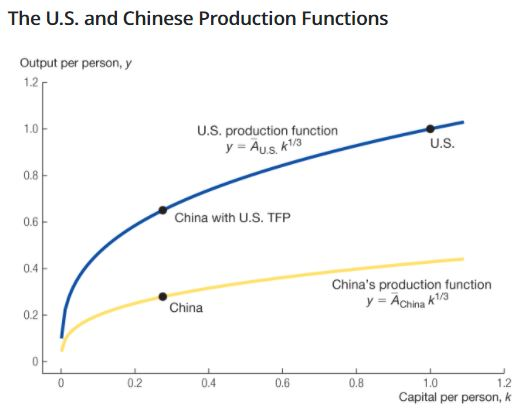
\includegraphics[scale=.62]{TFP_china_us}
\end{figure}
\end{frame}

\begin{frame}
\frametitle{\: \: \: Understanding differences in $\overline{A}$}
\toplinelarge
\begin{figure}
\centering
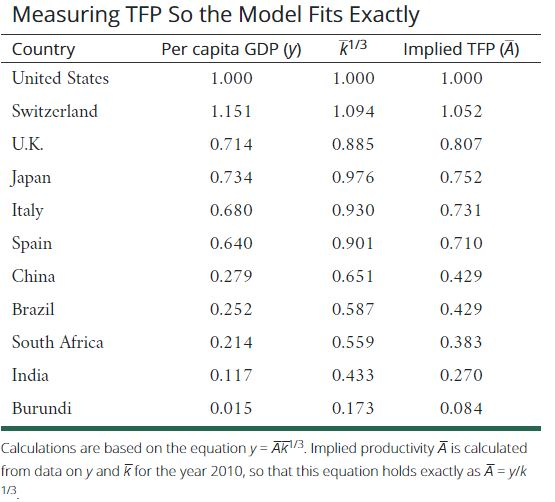
\includegraphics[scale=.58]{TFP_perfect_fit}
\end{figure}
\begin{itemize}
\item In general, $67\%$ of variation is explained by differences in $\overline{A}$  and  $33\%$ by differences in $k$.  
\end{itemize}
\end{frame}

\begin{frame}
\frametitle{\: \: \: Understanding differences in $\overline{A}$}
\toplinelarge
\begin{itemize}
\item A common interpretation of differences in $\overline{A}$ is differences in Total Factor Productivity (TFP)
\begin{itemize}
\vspace{.11in}
\item Some countries have high $y$ because of large reserves of natural resources (e.g. oil rich countries), but usually is due to large factor productivity.
\end{itemize}
\vspace{.11in}
\item Important factors that have been shown to account for $TFP$ differences across countries are:
\begin{enumerate}
\vspace{.11in}
\item Differences in Human Capital
\vspace{.11in}
\item Differences in Technology
\vspace{.11in}
\item Differences in Institutions that promote economic growth
\vspace{.11in}
\item Missallocation of production resources 
\end{enumerate}
\end{itemize}
\end{frame}

\section{The Solow Growth Model}

\begin{frame}
\frametitle{\: \: \: Introduction}
\toplinemedium
\begin{itemize}
\item The production model is very useful because is able to display two features of the data:
\begin{enumerate}
\vspace{.11in} 
\item $\frac{y_{ind}}{y_{nind}}=\frac{\overline{A}_{ind} \left(\overline{k}_{ind}\right)^{\frac{1}{3}}}{\overline{A}_{nind} \left(\overline{k}_{nind}\right)^{\frac{1}{3}}}$ (differences in levels of $y$)  
\vspace{.2in} 
\item $g_{y_{ind}}-g_{y_{nind}}=(g_{\overline{A}_{ind}}+\frac{1}{3} g_{\overline{k}_{ind}})-(g_{\overline{A}_{nind}}+\frac{1}{3}g_{\overline{k}_{nind}})$ (differences in growth rates of $y$)  
\end{enumerate}
\vspace{.11in} 
\item Nevertheless, it does not provide any explanation as to why the growth rates are so different across countries.
\begin{itemize}
\vspace{.11in} 
\item The Solow Model provides an explanation for $K$ accumulation, which will help us to explain why capital per worker grows at a faster pace in some countries.
\vspace{.11in} 
\item As we have seen this is only a part of the explanation, but it is a very useful starting point for understanding the big differences in growth rates we observe in the data.   
\end{itemize}
\end{itemize}
\end{frame}

\begin{frame}
\frametitle{\: \: \: Capital Accumulation}
\toplinemedium
\begin{itemize}
\item At the center of the Solow Model is the capital accumulation equation:
\begin{eqnarray*}
K_{t+1}=I_t+(1-\overline{d})K_t
\end{eqnarray*}
\begin{itemize}
\item $I$=investment, $\overline{d}$=depreciation rate ($0 \leq \overline{d} \leq 1$)
\end{itemize}
\vspace{.11in}
\item We can rewrite this equation in changes: $\Delta K_{t+1}=K_{t+1}-K_t$:
\begin{columns}
\begin{column}{0.4\linewidth}
\begin{eqnarray*}
\Delta K_{t+1}=I_t-\overline{d}K_t:
\end{eqnarray*}
\end{column}
\begin{column}{0.7\linewidth}
\begin{figure}
\centering
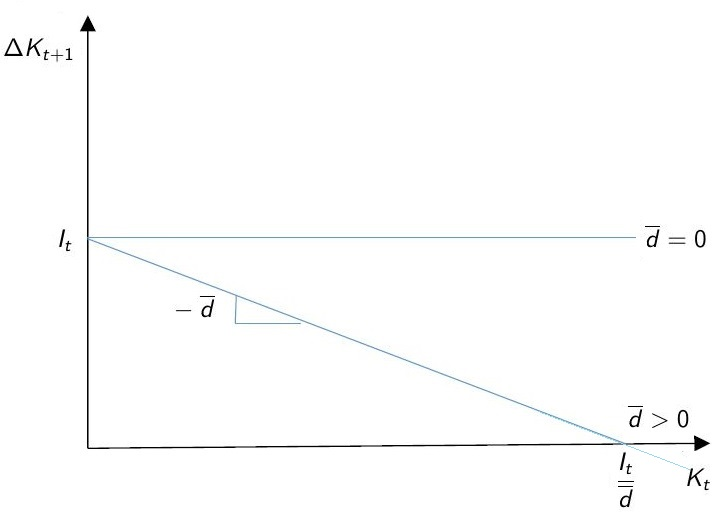
\includegraphics[scale=.28]{lom}
\end{figure}
\end{column}
\end{columns}
\end{itemize}
\end{frame}

\begin{frame}
\frametitle{\: \: \: Capital Accumulation}
\toplinemedium
\begin{itemize}
\item Investing in capital for $t+1$ requires resources at $t$:
\begin{eqnarray*}
C_t+I_t=Y_t \: \: \: \: \: (\text{resource constraint})
\end{eqnarray*}
\begin{itemize}
\item An assumption of the Solow model is that capital and consumption goods are produced using the same production function.
\vspace{.11in}
\end{itemize}
\item We are going to assume that individual decisions to save and invest is exogenous:
\begin{eqnarray*}
\begin{array}{lcl}
I_t=\overline{s} Y_t \: \: \: \: \: (\text{allocation of resources}) &,&0 \leq \overline{s} \leq 1
\end{array} 
\end{eqnarray*}
\item Combining the allocation of resources with the capital accumulation equation, we obtain:
\only<1>{\begin{eqnarray*}
\Delta K_{t+1}=\overline{s} Y_t-\overline{d}K_t \: \: \: \: \: (\text{law of motion})
\end{eqnarray*}}
\only<2>{\begin{eqnarray*}
\Delta K_{t+1}=\overline{s} F(K_t,L_t)-\overline{d}K_t \: \: \: \: \: (\text{law of motion})
\end{eqnarray*}}
\end{itemize}
\end{frame}

\begin{frame}
\frametitle{\: \: \: Dynamics of Capital Accumulation}
\toplinexlarge
\only<1>{\begin{figure}
\centering
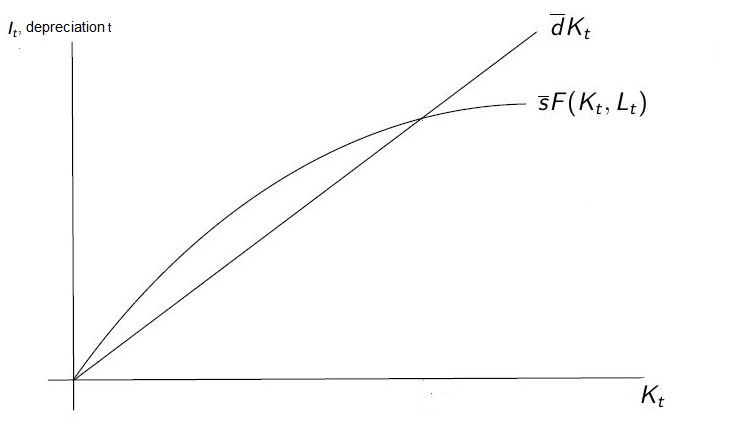
\includegraphics[scale=.6]{basic_solow}
\caption{$\Delta K_{t+1}=\overline{s} F(K_t,L_t)-\overline{d}K_t $}
\end{figure}}
\only<2>{\begin{figure}
\centering
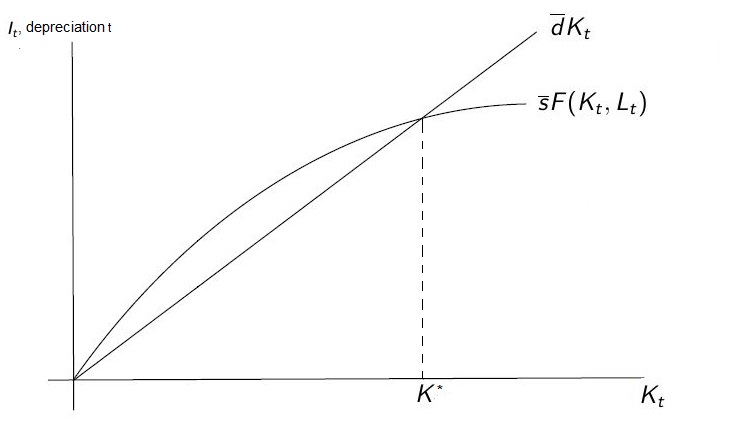
\includegraphics[scale=.6]{basic_solow_2}
\caption{$\underbrace{\Delta K_{t+1}}_{K_{t+1}=K_t}=0  \Leftrightarrow  \underbrace{\overline{s}F(K_t,L_t)}_{I_t}=\overline{d}K_t$}
\end{figure}}
\only<3>{\begin{figure}
\centering
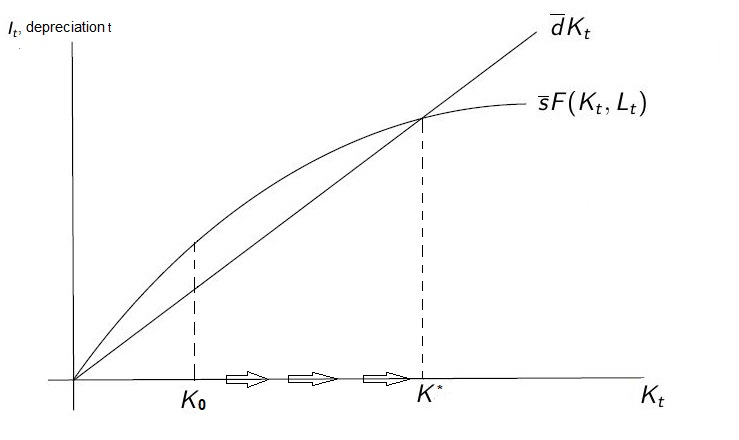
\includegraphics[scale=.6]{basic_solow_3}
\caption{$\underbrace{\Delta K_{t+1}}_{K_{t+1}>K_t}>0  \Leftrightarrow  \underbrace{\overline{s}F(K_t,L_t)}_{I_t}>\overline{d}K_t$}
\end{figure}}
\only<4>{\begin{figure}
\centering
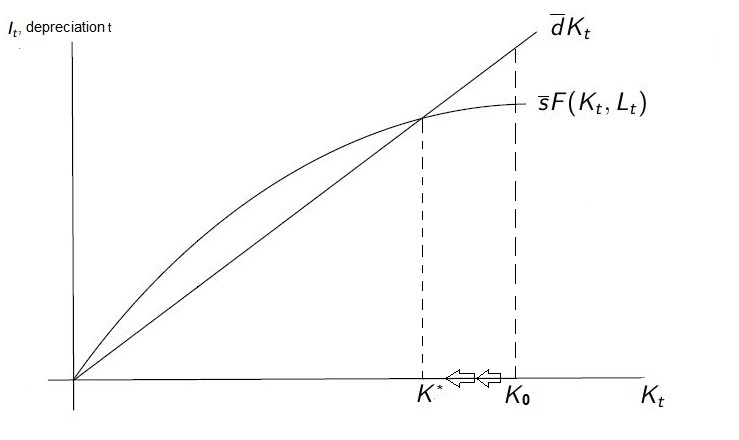
\includegraphics[scale=.6]{basic_solow_4}
\caption{$\underbrace{\Delta K_{t+1}}_{K_{t+1}<K_t}<0 \Leftrightarrow  \underbrace{\overline{s}F(K_t,L_t)}_{I_t}<\overline{d}K_t$}
\end{figure}}
\end{frame}





\end{document}